\begin{frame}
\frametitle{Introductory Calculus--Infinitesimal Approach}
\framesubtitle{1.4 More Properties of Hyperreals And Infinitesimals}
\label{slide:1.4-07}
\begin{itemize}
\item<1->
Hyperreal Numbers Which Are Not Infinite, Are \alert{Finite Numbers}.
\item<2->
About each $c\in\mathbb{R}$ Is \alert{A Portion of Hyperreal Line Composed of The Numbers Infinitely Close to $c$}.
\visible<2->
{
\begin{figure}[H]
\centering
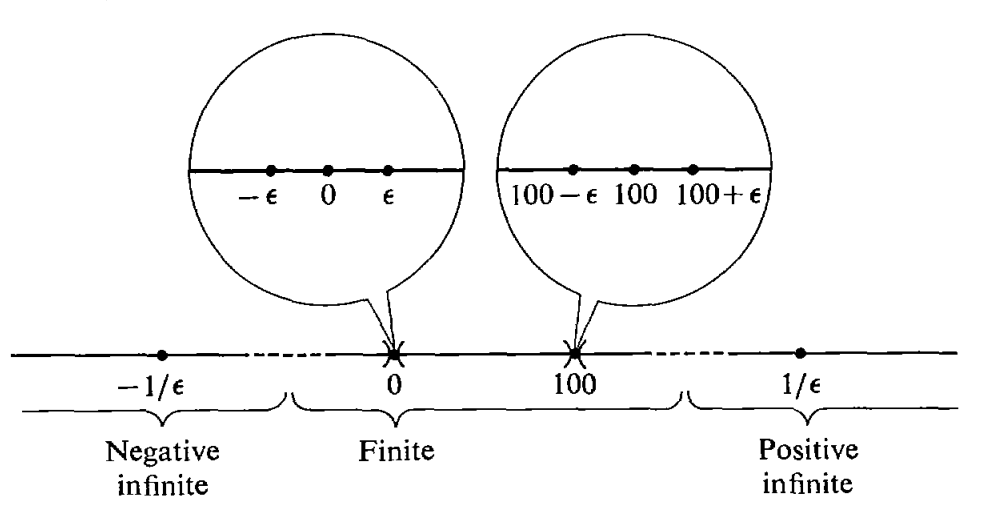
\includegraphics[width=.5\textwidth]{images/infinitesimal-microscope}
\caption{Finite And Infinite Parts of The Hyperreal Line (\textit{Infinitesimal Microscope} about $c=0,c=100$)}
\label{fig:finfinhyperreal}
\end{figure}
}
\item<3->
\alert{Numbers Infinitely Close to $0$ Are Infinitesimals}.
\end{itemize}
\end{frame}
